\chapter{Design}

\section{The Physical Prototype}

The prototype consists of a lightweight box which can be easily assembled and disassembled, of which four sides are laser cut MDF and the top is a square piece of plexiglass. The bottom is open. A number of tokens may be moved around the surface of the box. The tokens are circular and 3D printed, with a colored marker on the bottom and a picture of the token's virtual counterpart on the top. A camera is placed at the bottom of box, looking up. A light is placed next to the camera, shining on the side of the box to create a diffused light. 
The setup is connected to an HTC Vive with no modifications.

\subsection{The box}

The construction of the box consists of four identical sides measuring 570 by 300 by 300 mm. MDF (medium-density fibreboard) was chosen for the box as it is lightweight, sturdy, and easy to cut with a laser cutter. It is important that the prototype is lightweight as it must be transported to various locations for testing. The precise laser cutting of the sides means that the sides can be made with the interlocking parts that connect firmly without the need for mechanical locking parts. The main concern was ensuring the pieces form a tight fit. Since material is removed during the laser cutting process, the design had to be purposely made too tight. The test cut worked well at first, but the fit became too loose after being put together and taken apart a few times. A tighter fit was then designed for the final cut of the prototype elements. If the prototype experiences the same issue, we must attach hasps or a similar solution to keep the sides from coming apart. 

The bottom of the box is left open for an easier setup.
The box is made to be tall enough that the camera can capture all of the plexiglass surface in its field of view, which we determined was 570 mm.
The construction was designed to be rectangular as this is the shape of the average garden. %citation needed
%30,30,57 and 297
The top of plexiglass is needed so that there is a place to put the tokens, which the camera can see. Acrylic was considered, but was too expensive for this project as only quite large sizes were available.

The plexiglass top of the box is a square, made to be fitted into the box, resting on wooden strips glued to the sides of the box. The strips are to be no more than a centimeter wide. Ideally notches would be cut into the plexiglass and the top of the sides of the box, allowing us to simply lock the top into place without the need for the wooden strips. This was however first thought of after the sides had been cut. Adding the additional cuts to the sides would be tricky to do with perfect accuracy, as even a slight error would ruin the fit. 
Holes are cut into the sides near the bottom to route cables for the webcam through, while doubling as carrying handles for easy transportation. 

\subsection{The tokens}

The physical construction of the tokens was not a cause of great concern. They simply needed to be circular. We chose 3D printing for the tokens for consistency's sake, and for the easy of construction. The markers themselves are color prints on regular white printer paper, which are to be glued to the bottom of the tokens. Markers can be easily reprinted and replaced if a problem is found with the current image processing implementation. 
The size of the markers is made to be as small as possible while still working with the image processing aspect. It all depends on the quality of the webcam image. The worse quality the webcam delivers, the larger the markers need to be. With a proper DSLR camera we could scale down the markers considerably, but the software to make such a camera work as a webcam is expensive, and so for the prototype we went with a webcam.

The marker is designed to have a thick stroke around its perimeter. This is what makes the program classify it as a marker. At one point, a line is drawn from the edge of the marker and slightly inwards. This lets the program determine the token's rotation vector. In the center of the marker, between 0 and 8 squares are placed.
\begin{figure}[H]
	\centering
	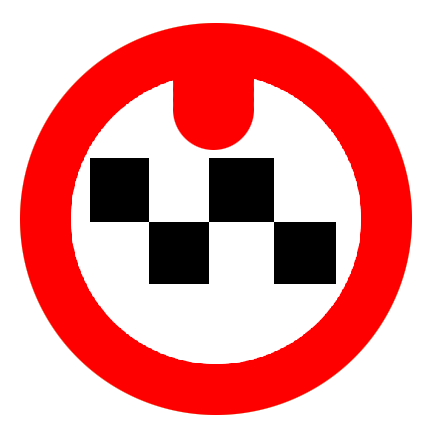
\includegraphics[width=0.3\linewidth]{figure/Analysis/circleexample2}
	\caption{Example marker indicating a value of 165}
	\label{fig:circle2}
\end{figure}

These each represent a bit, black indicating a 1 and white indicating a 0. They do not necessarily need to be square. The program looks at the center of each to get a brightness value.

\begin{figure}[H]
	\centering
	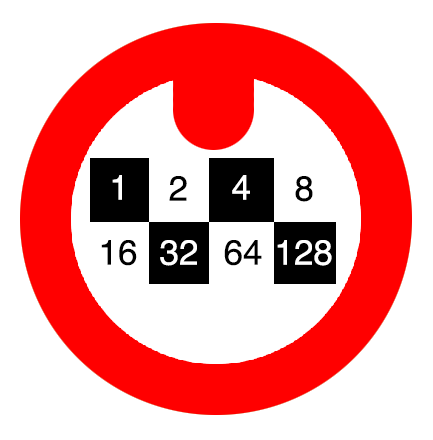
\includegraphics[width=0.3\linewidth]{figure/Analysis/circleexample}
	\caption{The value
		 each square represents}
	\label{fig:circle}
\end{figure}

This allows us to print a marker representing any one of 255 items. More could be added later, but for testing the prototype there is no need for more combinations as we are limited by the number of unique digital models.

A program was made to automatically generate markers as needed. It takes an array of integers and creates sheets of markers corresponding to the array. For the input \codeword{int[] markers = {1, 2, 4, 8, 16, 32, 64, 128, 100, 3, 9};} it returns the following image:

\begin{figure}[H]
	\centering
	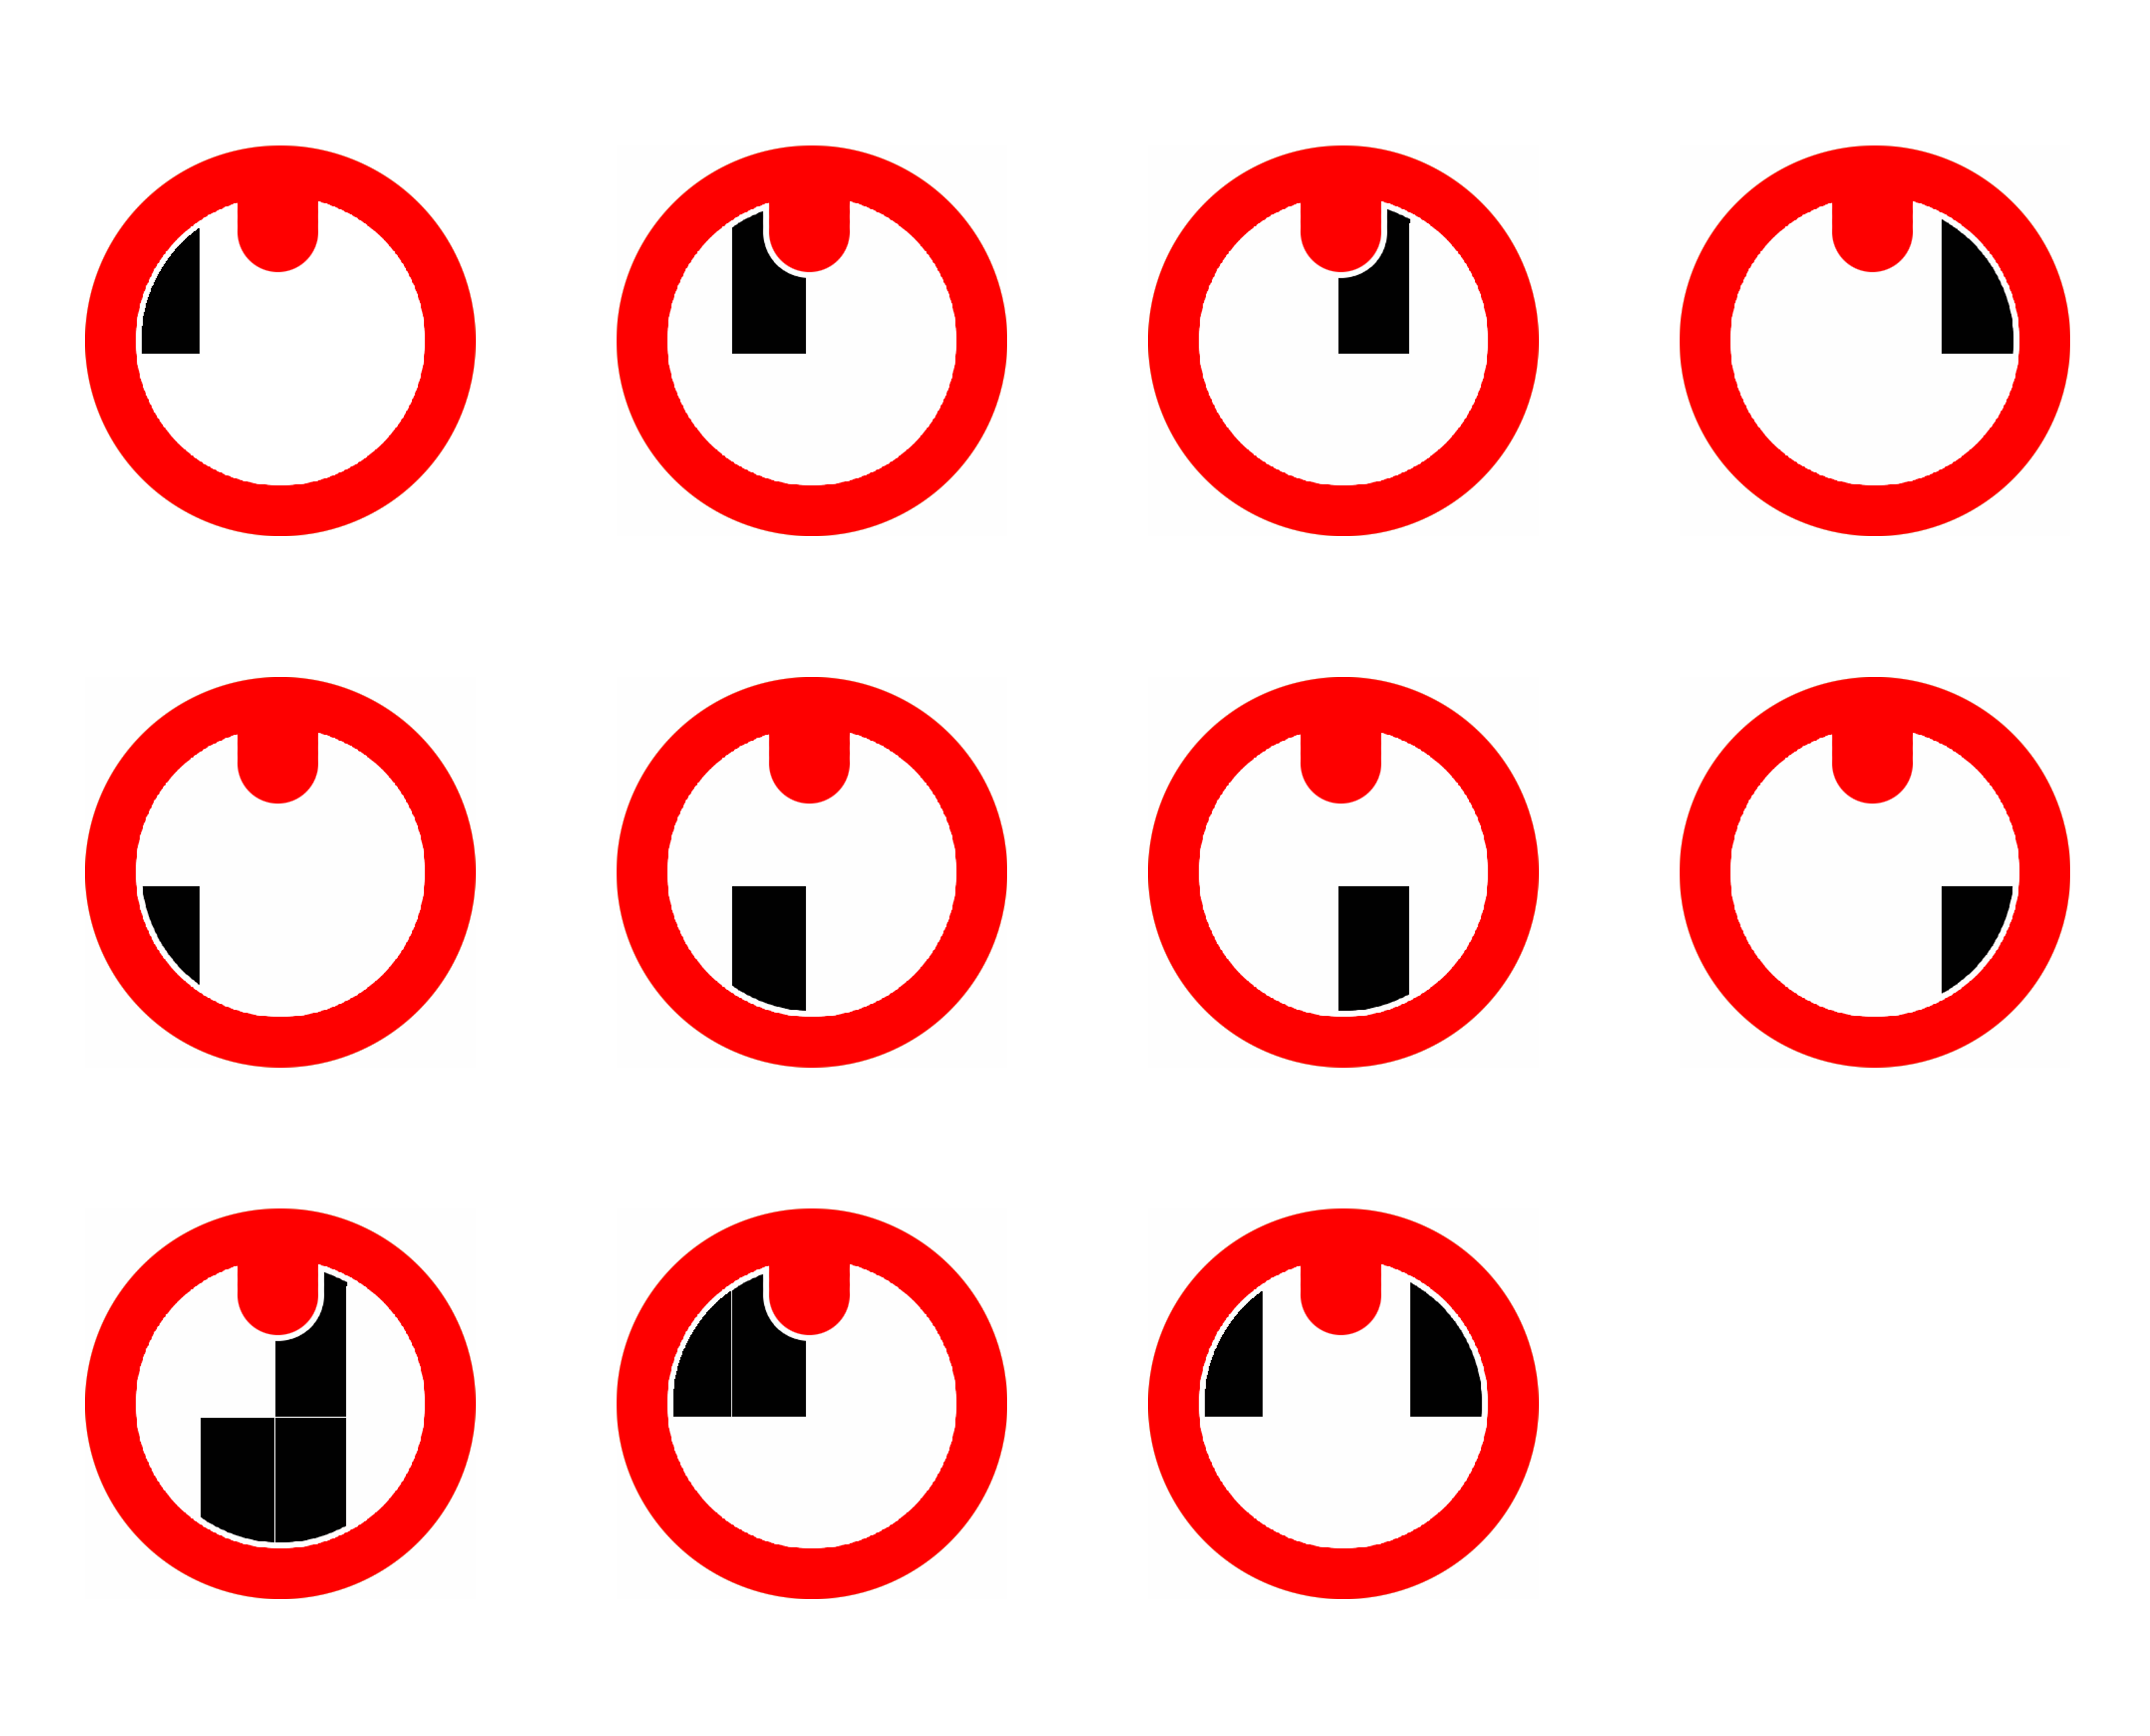
\includegraphics[width=0.6\linewidth]{figure/Analysis/result}
	\caption{Automatically generated markers}
	\label{fig:result}
\end{figure}


\section{The Virtual Environment}

\subsection{The UI}
Not much is needed in terms of a user interface. All manipulation of the virtual objects is done by moving around the physical tokens. All the user can do inside the virtual world is move around. The VR controller is visible as a model which looks exactly like the physical controller, to minimize confusion. The only added element is a highlight of the trackpad with the text "Teleport" beside it. This is added as there in an early test was a bit of confusion communicating which of the buttons allowed one to teleport around the environment.

\todo{Possibly add something about the 3D models - why were they designed the way they were?}